\section{Arkiektur}

Hardware arkitekturen er beskrevet ved domænemodel og BDD diagrammer, disse diagrammer bliver beskrevet her under for at skabe et overblik over systemets forbindelser.


\subsection{Domænemodel}

På figur \ref{fig:dmLAMP} er afbildet en domænemodel for hele systemet. Dette diagram hjælper til at skabe et overblik for virkemåden af systemet. De sorte pile på diagrammet beskriver en sammenhæng eller en handling der sker mellem blokkene, som er dele i systemet. I domænemodellen er der brugt talesprog for at sikre at en kommende bruger uden teknisk baggrund kan få et overblik over systemet.

\begin{figure}[H] \centering
    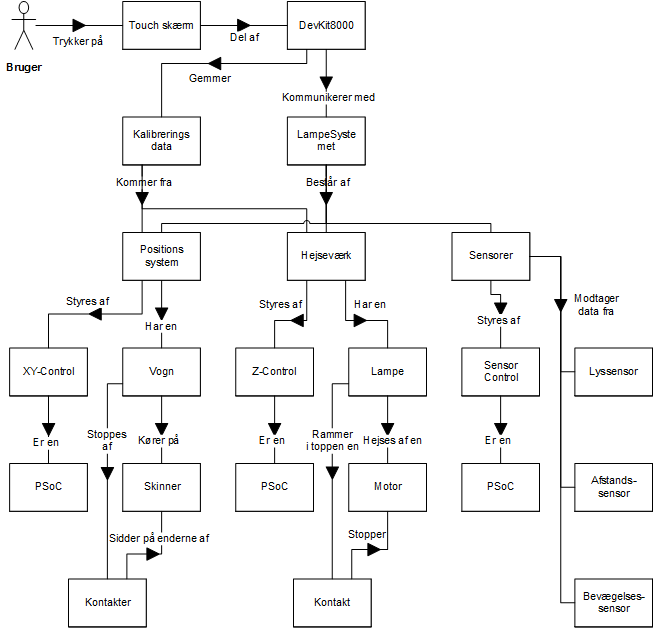
\includegraphics[width=\textwidth]{Filer/dmLAMP.png}
    \caption{Domænemodel L.A.M.P.}
    \label{fig:dmLAMP}
\end{figure}


\subsection{Blokdefinitionsdiagram}

På figur \ref{fig:bddLAMP} ses det overordnede BDD for systemet med de forskellige blokke det er blevet opdelt i. Et BDD er en overordnet beskrivelse af systemets blokke, med signaler, der går til og fra disse blokke. Derud over fremgår det hvordan blokkene er forbundet med hinanden.

\begin{figure}[H] \centering
    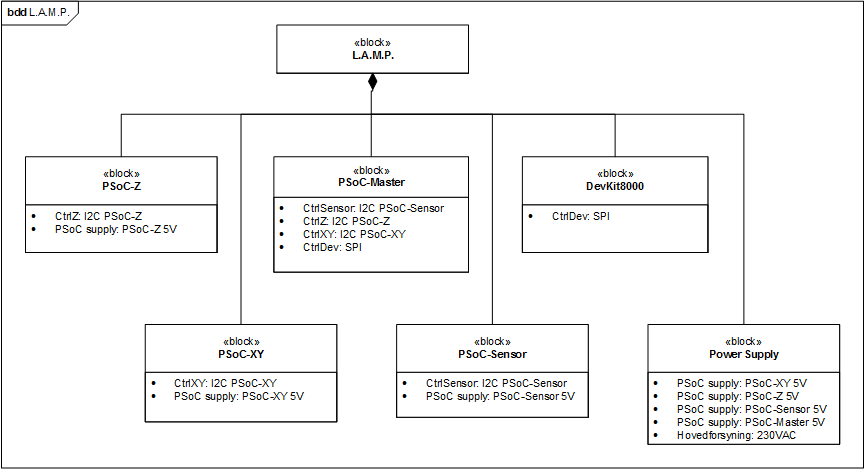
\includegraphics[width=\textwidth]{Filer/bddLAMPvers3.png}
    \caption{BDD L.A.M.P.}
    \label{fig:bddLAMP}
\end{figure}


\subsection{Intern blokdiagram}

På figur \ref{fig:ibdLAMP} ses IBD for det overordnede system. Her fremgår forbindelserne og signal navne mellem de forskellige blokke.

Som det fremgår af figur \ref{fig:ibdLAMP} er der 6 hovedblokke, som alle er en del af systemet L.A.M.P. Tre af disse blokke PSoC-XY, PSoC-Z og PSoC-Sensor består yderligere af dele som fremgår detaljeret af BDDer og IBDer i arkiteturdokumentet i bilag \footcite{documentation}.

\begin{figure}[H] \centering
    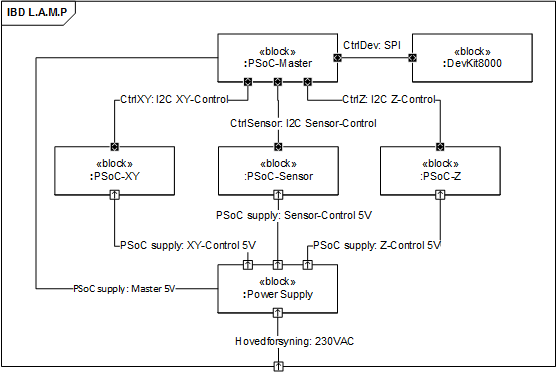
\includegraphics[width=\textwidth]{Filer/ibdLAMPvers3.png}
    \caption{IBD L.A.M.P.}
    \label{fig:ibdLAMP}
\end{figure}

\textbf{Beskrivelse af blokkene}

PSoC-Master: Denne blok står for al kommunikationen. Den modtager kommandoer fra DevKit8000 via SPI kommunikation. Disse kommandoer sender den via I2C kommunikation videre til den PSoC kommandoen omhandler.

PSoC-XY: Denne blok står for styringen af X og Y bevægelsen af systemet. Når den modtager en kommando fra PSoC-Masteren udføres den ønskede handling. 

PSoC-Z: Denne blok står for styringen af Z bevægelsen af systemet. Når den modtager en kommando fra PSoC-Masteren udføres den ønskede handling.

PSoC-Sensor: Denne blok styrer og bearbejder data fra sensorene og RGB-dioderne i systemet.

Power Supply: Som power supply til forsyning af systemet bruges en USB-hub som kan forsyne alle 4 PSoCs.

DevKit8000: Denne blok består af et bruger interface, det er her brugeren kan, via en touchskærm, sende ønskede kommandoer til systemet. 
